% !TEX TS-program = xepythontex

\documentclass[10pt, envcountsect , spanish]{beamer}


\newif\ifnotas
\notasfalse% Para no mostrar los globos
\notastrue % Para  mostrar los globos

\input ../preambulo.tex

\usepackage[normalem]{ulem}               % to striketrhourhg text
\newcommand\tacha{\bgroup\markoverwith{\textcolor{black}{\rule[0.5ex]{2pt}{0.8pt}}}\ULon}






%································ TITULO, AUTOR, ETC


\title[Interfaces de Usuario]{Interfaces de Usuario}
%\subtitle{}

\author[L. Daniel Hernández]{L. Daniel Hernández $<ldaniel@um.es>$}

\institute[ldaniel@um.es]{Dpto. Ingeniería de la Información  y las Comunicaciones\\ Universidad de Murcia \\ 4 de diciembre de 2023\newline \hrule}


\date[ldaniel@um.es]{ 
\vskip 1.0cm
%\vskip -1.25cm
%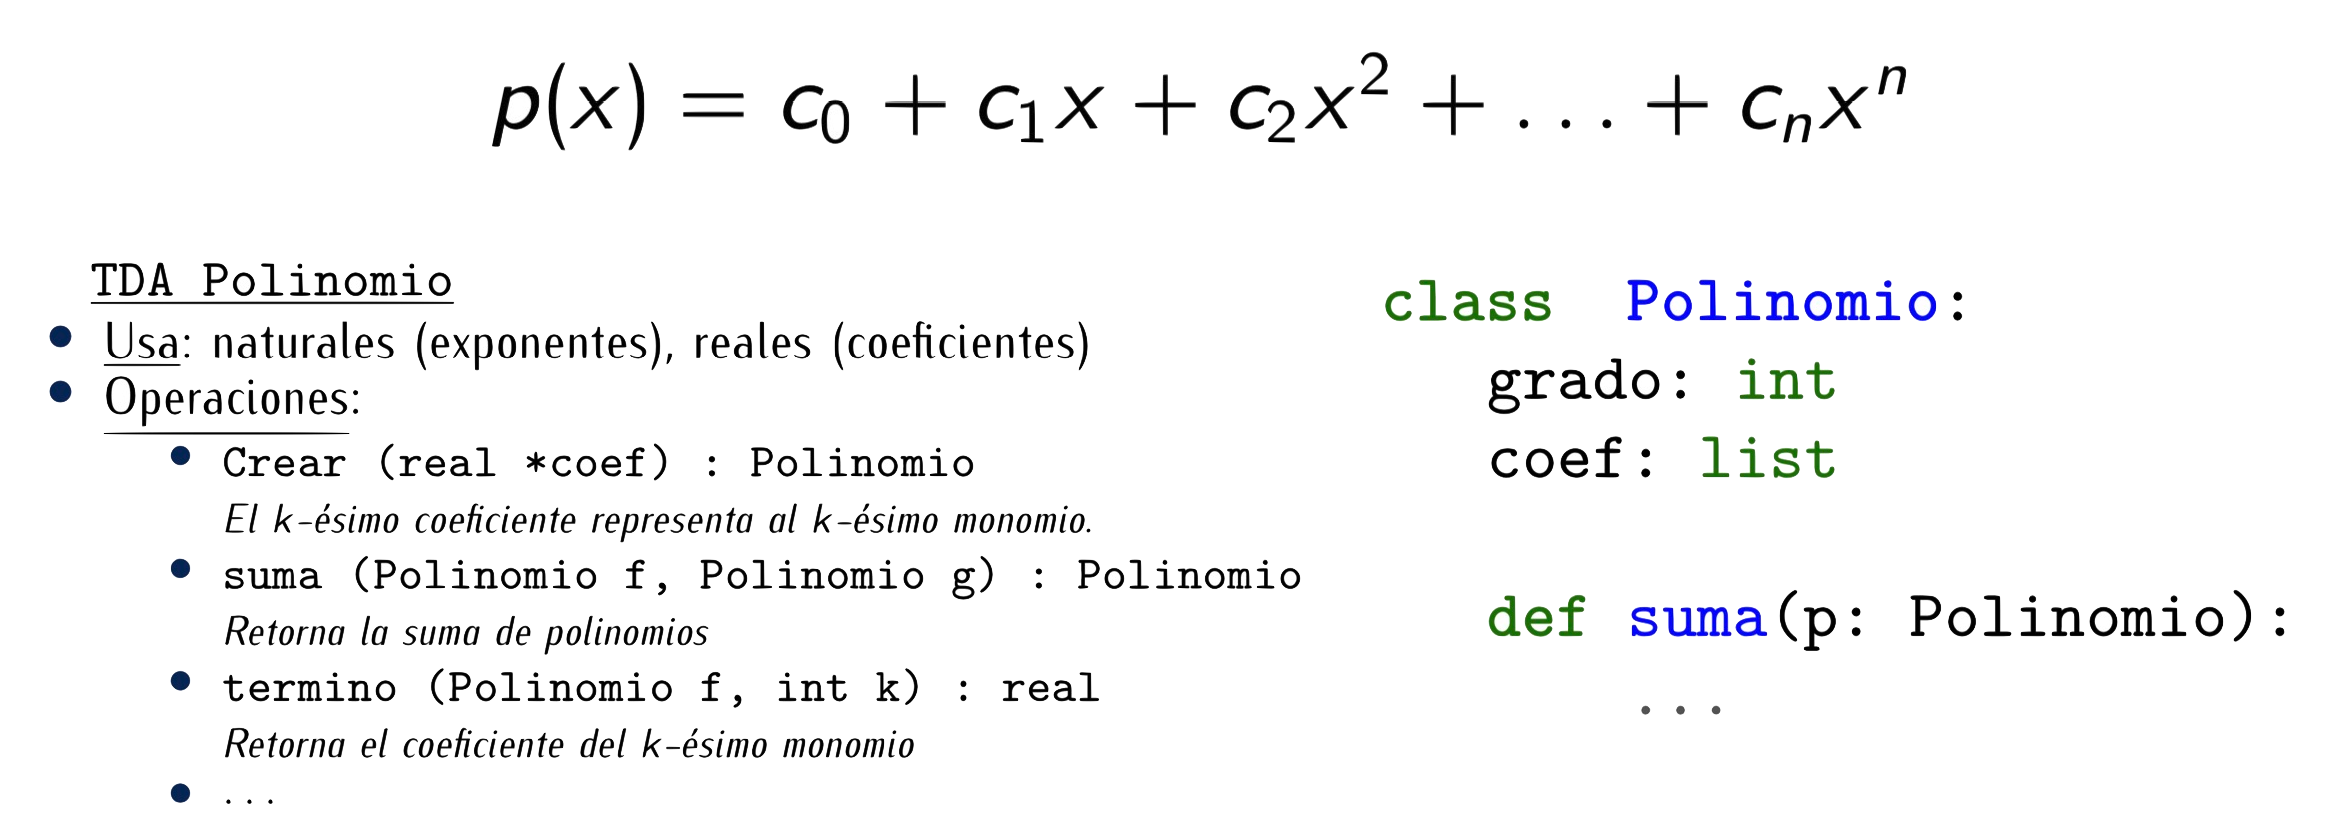
\includegraphics[width=.8\textwidth, height=.18\textheight]{fig/polinomio}
}

\graphicspath{{img/}}






%%%%%%%%%%%%%%%%%%%%%%%%%%%%%%%%%%
%%%%%%%%%%%%%%%%%%%%%%%%%%%%%%%%%%
%%%%%%%%%%%%%%%%%%%%%%%%%%%%%%%%%%
%%%%%%%%%%%%%%%%%%%%%%%%%%%%%%%%%%

%https://es.overleaf.com/learn/how-to/Writing_Markdown_in_LaTeX_Documents
\usepackage[hashEnumerators]{markdown}


%%%%%%%%%%%%%%%%%%%%%%%%%%%%%%%%%%
%%%%%%%%%%%%%%%%%%%%%%%%%%%%%%%%%%
%%%%%%%%%%%%%%%%%%%%%%%%%%%%%%%%%%
%%%%%%%%%%%%%%%%%%%%%%%%%%%%%%%%%%
\begin{document}

%\pgfdeclareimage[height=1cm]{logo}{logo.png}
%\logo{\pgfuseimage{logo}}



%--------------------------------------------------------------------------------
{\usebackgroundtemplate{%
  \includegraphics[width=\paperwidth,height=\paperheight]{../img/fondoUMUCompleto}}

\begin{frame}[b]
	\maketitle

\begin{tikzpicture}[overlay, remember picture]
\node[anchor=south west, %anchor is bottom left corner of the graphic
      xshift=.32\textwidth, %shifting around
      yshift=0.7cm] 
     at (current page.south west) %left bottom corner of the page
     {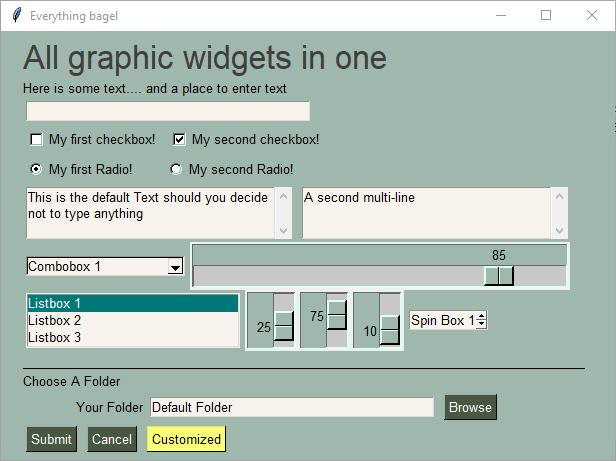
\includegraphics[width=.52\textwidth, height=.34\textheight]{fig/all-in-one}
     \footnote[frame]{\tiny
 Imagen: \url{https://www.ntu.edu.sg/home/ehchua/programming/java/J4a_GUI.html}  }}; 
\end{tikzpicture}
	
\end{frame}			% Transparencia: Título
}



%%%%%%%%%%%%%%%%%%%%%%%%%%%%%%%%%%%%%%%%%%%%%%%%
%%%%%%%%%%%%%%%%%%%%%%%%%%%%%%%%%%%%%%%%%%%%%%%%
\begin{frame}{Índice de Contenidos}\tableofcontents \end{frame}




%%%%%%%%%%%%%%%%%%%%%%%%%%%%%%%%%%%%%
%%%%%%%%%%%%%%%%%%%%%%%%%%%%%%%%%%%%%
\section{Interface Gráficas de Usuario}


%%%%%%%%%%%%%%%%%%%%%%%%%%%%%%%%%%%%%
%%%%%%%%%%%%%%%%%%%%%%%%%%%%%%%%%%%%%
\begin{frame}{GUIs en Python} 
\begin{itemize}
\item No hay que confundir las herramientas de GUI con herramientas de gráficos o herramientas de visualización de datos.
\item \key{Tkinter} es un \textit{binding} de Python al kit de herramientas de la GUI de Tk. 
\item \key{Tk} es la biblioteca GUI original para el lenguaje Tcl. 
\item Tkinter se implementa como un envoltorio (\textit{wrapper}) de Python alrededor de un intérprete de Tcl completo incrustado en el intérprete de Python. 
\item Otros lenguajes que usan Tk son: Tcl, Ruby, Perl.
\item Hay \key{otras librerías} de GUI para Python: wxPython, PyQt y PyGTK.
\item Python ya tiene construidas algunas GUI por nosotros.
\item Lo normal es que construyamos también nuestra propia GUI.
\end{itemize}
\end{frame}



%%%%%%%%%%%%%%%%%%%%%%%%%%%%%%%%%%%%%
%%%%%%%%%%%%%%%%%%%%%%%%%%%%%%%%%%%%%
\section{Conceptos Básicos}

%%%%%%%%%%%%%%%%%%%%%%%%%%%%%%%%%%%%%
%%%%%%%%%%%%%%%%%%%%%%%%%%%%%%%%%%%%%
\begin{frame}[fragile]{Conceptos Tk} {\url{https://docs.python.org/3.9/library/tkinter.html\#tkinter.Tk}}
\begin{itemize}
\item\key{ Widget: }
\begin{itemize}
\item Es cualquier objeto que represente a un elemento de la ventana (botones, frames, ...)
\item Crear un widget es crear un objeto de una clase específica.
\item Todos los widget forman parte de un árbol jerárquico de widget.
\footnotesize
\begin{pyverbatim}[][frame=single]
root = Tk()  #  root es la ventana principal
root.title("Título de la ventana")
# root.resizable(True, False)
# root.geometry("720x350")
# Crear árbol jerárquico
root.mainloop()
\end{pyverbatim}
\end{itemize}

\item \key{Geometry Manager: }
\begin{itemize}
\item Es el encargado de indicar exactamente dónde se colocará cada widget.
\item Trabaja con widgets  master (maestro) y slave (esclavo)
\item Un widget maestro suele hacer referencia a una ventana o marco que contiene widgets esclavos.
\end{itemize}

\item \key{Event Handling:}  
\begin{itemize}
\item Tk ejecuta un bucle de eventos que recibe eventos del sistema operativo (pulsaciones de teclas, movimiento del ratón, cambio de tamaño en la ventana, etc).
\item Cuando se recibe un evento, el widget afectado invocará a un comando.

\footnotesize
\begin{pyverbatim}[][frame=single]
tk.Button(mainframe, text="Calculate", command=calculate)
\end{pyverbatim}
\end{itemize}

\end{itemize}
\end{frame}




%%%%%%%%%%%%%%%%%%%%%%%%%%%%%%%%%%%%%
%%%%%%%%%%%%%%%%%%%%%%%%%%%%%%%%%%%%%
\begin{frame}[fragile]{Variables de Control}

\begin{itemize}
\item Las variables de control son objetos que se asocian a los widgets.
	\begin{itemize}
	\item Estas variables almacenan valores del widget para que estén disponibles en otras partes del programa.
	\item Cuando cambian sus valores queda reflejado de forma automática en el widget.
	\end{itemize}
\item Hay cuatro tipos:
\begin{pyverbatim}[][frame=single]
entero   = IntVar()      # Para trabajar con enteros
real     = DoubleVar()   # Para usar números de tipo flotante
cadena   = StringVar()   # Para usar cadenas de caracteres
booleano = BooleanVar()  # Para trabajar con booleanos.
\end{pyverbatim}
\item Métodos:
\begin{itemize}
\item \cm{.set(valor)}, asigna un valor a la variable de control.
\item \cm{.get()}, retorna el valor de la variable de control.
\item \cm{.trace(tipo, función)}, se emplea para detectar cuándo la variable es leída, cambia su valor o es borrada.
	\begin{itemize}
	\item \cm{tipo}, indica el tipo de suceso a comprobar: 'r', lectura de variable; 'w', escritura de variable, 'u', borrado de variable.
	\item \cm{función} indica la función que será llamada cuando ocurra el suceso.
	\end{itemize}
\end{itemize}
\end{itemize}
\end{frame}







%%%%%%%%%%%%%%%%%%%%%%%%%%%%%%%%%%%%%
%%%%%%%%%%%%%%%%%%%%%%%%%%%%%%%%%%%%%
\begin{frame}{Construcción de Variables de Control y Ejemplo de Uso}


\begin{itemize}
\item Constructor: {\small \pyv{var = tk.xxxVar (contenedor, valor, nombre)}}

	\begin{itemize}
	\item Son 3 parámetros opcionales.
	\item \cm{contenedor}: es un widget asociado con el objeto xxxVar. 
		Si se omite el contenedor, el valor predeterminado es la ventana raíz.
	\item \cm{valor}: es el valor inicial que por defecto es una cadena vacía \cm{''}.
	\item \cm{nombre}: es un nombre de Tcl que por defecto es \pyv{PY_VARnum}.
	\end{itemize}
	
\item Un ejemplo de uso\footnote{\url{https://www.pythontutorial.net/tkinter/tkinter-stringvar/}}:
	\begin{itemize}
	\item \cm{StringVar} administra el valor de un widget, como una etiqueta o una entrada.
	\item Después de crear el objeto StringVar, puedes \key{asignarlo a la variable de texto}, \pyv{text}, de un widget que acepta un objeto StringVar.
	\item \pyv{string_var.get()} retorna el valor actual del  \pyv{string_var}
	\end{itemize}

\item[] \unEjemplo
	\begin{itemize}
	\item \pyv{Label(parent, text=string_var.get())}
	\item \pyv{Entry(parent, text=string_var)}
	\end{itemize}
	
\end{itemize}
\end{frame}







%%%%%%%%%%%%%%%%%%%%%%%%%%%%%%%%%%%%%
%%%%%%%%%%%%%%%%%%%%%%%%%%%%%%%%%%%%%
\section{Ventanas de Mensajes}




%%%%%%%%%%%%%%%%%%%%%%%%%%%%%%%%%%%%%
%%%%%%%%%%%%%%%%%%%%%%%%%%%%%%%%%%%%%
\begin{frame}{Tkinter Dialogs} {\url{https://docs.python.org/3.9/library/tkinter.messagebox.html}}


\begin{itemize}
\item
El módulo \cm{tkinter.messagebox} crea ventanas de  mensaje  modales.

\item messagebox\cm{.Message(master=None, **options)} crea una ventana de mensaje de información por defecto.

\item Pero se pueden concretar aún más:

\begin{itemize}
\item Mensaje de información:
	\begin{itemize}
	\item messagebox\cm{.showinfo()}
	\end{itemize}
	
\item Mensajes de aviso
	\begin{itemize}
	\item messagebox\cm{.showwarning()}
	\item messagebox\cm{.showerror()}
	\end{itemize}

\item Mensajes de preguntas
	\begin{itemize}
	\item messagebox\cm{.askquestion()}
	\item messagebox\cm{.askokcancel()}
	\item messagebox\cm{.askretrycancel()}
	\item messagebox\cm{.askyesno()}
	\item messagebox\cm{.askyesnocancel()}
	\end{itemize}
\end{itemize}

\end{itemize}
\end{frame}




%%%%%%%%%%%%%%%%%%%%%%%%%%%%%%%%%%%%%
%%%%%%%%%%%%%%%%%%%%%%%%%%%%%%%%%%%%%
\subsection{tkinter.messagebox.show\_\_\_}

%%%%%%%%%%%%%%%%%%%%%%%%%%%%%%%%%%%%%
%%%%%%%%%%%%%%%%%%%%%%%%%%%%%%%%%%%%%
\begin{frame}[fragile]{messagebox para mostrar información} 

\begin{pyverbatim}[][frame=single]
from tkinter import messagebox

messagebox.showinfo("Information", "Informative message")
messagebox.showerror("Error", "Error message")
messagebox.showwarning("Warning", "Warning message")
\end{pyverbatim}

\centerline{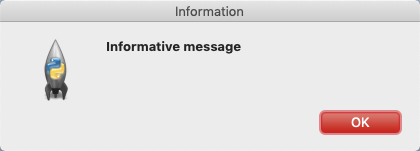
\includegraphics[width=.3\textwidth]{fig/showinfo} \hfill
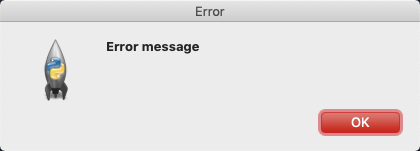
\includegraphics[width=.3\textwidth]{fig/showerror} \hfill
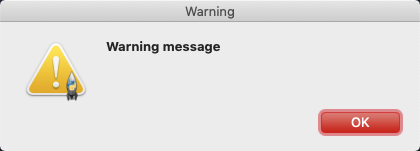
\includegraphics[width=.3\textwidth]{fig/showwarning}
}

\end{frame}




%%%%%%%%%%%%%%%%%%%%%%%%%%%%%%%%%%%%%
%%%%%%%%%%%%%%%%%%%%%%%%%%%%%%%%%%%%%
\subsection{tkinter.messagebox.ask\_\_\_}

%%%%%%%%%%%%%%%%%%%%%%%%%%%%%%%%%%%%%
%%%%%%%%%%%%%%%%%%%%%%%%%%%%%%%%%%%%%
\begin{frame}[fragile]{messagebox para pedir información} 

\footnotesize
\begin{pyverbatim}[][frame=single]
from tkinter import messagebox
answer = messagebox.askokcancel("Question", "Do you want to open this file?")
# False, True
answer = messagebox.askretrycancel("Question", "Do you want to try that again?")
# False, True
answer = messagebox.askyesno("Question", "Do you like Python?")
# False, True
answer = messagebox.askyesnocancel("Question", "Continue playing?")
# None, False, True
\end{pyverbatim}

\centerline{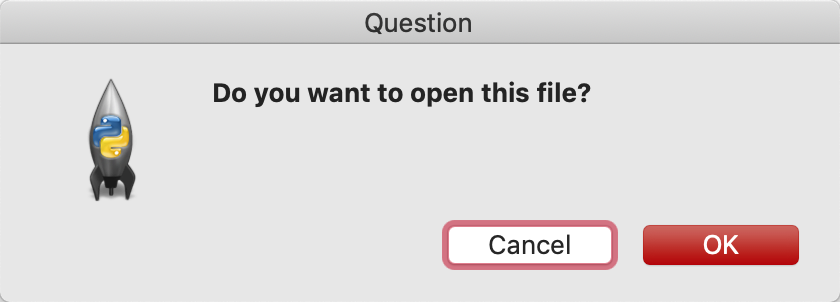
\includegraphics[width=.45\textwidth]{fig/askokcancel} \hfill
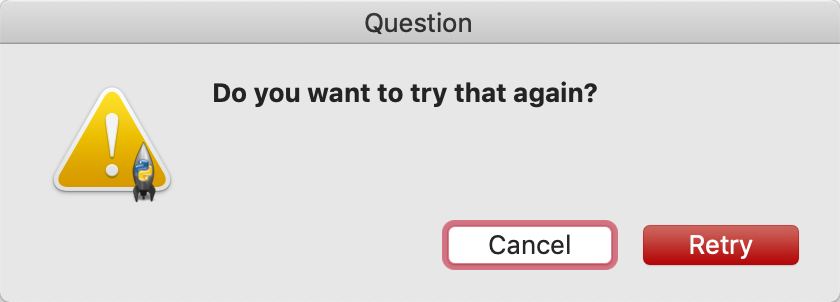
\includegraphics[width=.45\textwidth]{fig/askretrycancel}
}

\centerline{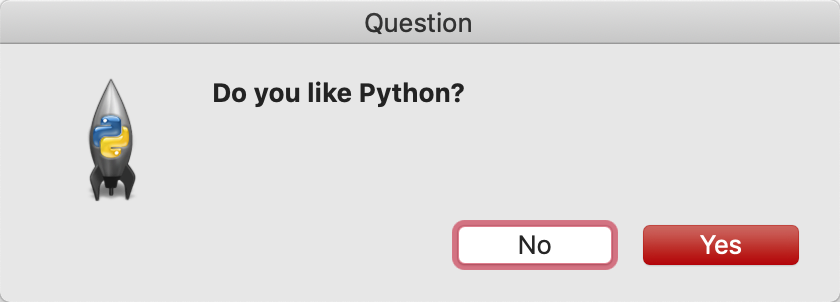
\includegraphics[width=.45\textwidth]{fig/askyesno} \hfill
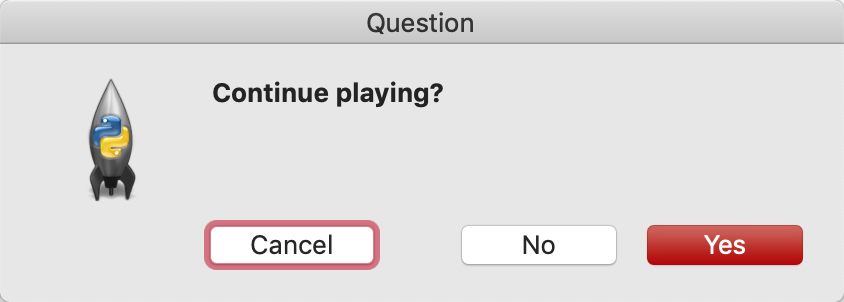
\includegraphics[width=.45\textwidth]{fig/askyesnocancel}
}

\end{frame}



%%%%%%%%%%%%%%%%%%%%%%%%%%%%%%%%%%%%%
%%%%%%%%%%%%%%%%%%%%%%%%%%%%%%%%%%%%%
\section{Ventanas de diálogo en tkinter}



%%%%%%%%%%%%%%%%%%%%%%%%%%%%%%%%%%%%%
%%%%%%%%%%%%%%%%%%%%%%%%%%%%%%%%%%%%%
\begin{frame}{Tkinter Dialogs} {\url{https://docs.python.org/3.9/library/dialog.html}}



\begin{description}


\item[tkinter.filedialog] File selection dialogs

\begin{itemize}
\item
Proporcionan \key{ventanas de diálogo para archivos} que combinan una apariencia nativa con opciones de configuración para personalizar el comportamiento. 

\item
Los siguientes argumentos  son aplicables a las clases y funciones de este módulo:

\begin{itemize}
\item 
parent:  la ventana para colocar el diálogo encima de
\item 
title: el título de la ventana
\item 
initialdir: el directorio en el que comienza el cuadro de diálogo
\item 
initialfile: el archivo seleccionado al abrir el cuadro de diálogo
\item 
filetypes: una secuencia de tuplas (etiqueta, patrón), se permite el comodín "*"
\item 
defaultextension: extensión predeterminada para agregar al archivo (guardar cuadros de diálogo)
\item 
multiple: cuando es verdadero, se permite la selección de varios elementos
\end{itemize}

\end{itemize}


\item[tkinter.simpledialog] Standard Tkinter input dialogs

\begin{itemize}
\item
Contiene clases y funciones adecuadas para crear \key{diálogos  simples}   para obtener un valor del usuario.

\item No olvides indicar a la ventana padre.
\end{itemize}


\end{description}
\end{frame}




%%%%%%%%%%%%%%%%%%%%%%%%%%%%%%%%%%%%%
%%%%%%%%%%%%%%%%%%%%%%%%%%%%%%%%%%%%%
\subsection{tkinter.filedialog}


%%%%%%%%%%%%%%%%%%%%%%%%%%%%%%%%%%%%%
%%%%%%%%%%%%%%%%%%%%%%%%%%%%%%%%%%%%%
\begin{frame}[fragile]{filedialog para Localizar un  Fichero} 
\footnotesize
\begin{pyverbatim}[][frame=single]
from tkinter import filedialog

fichero = filedialog.askopenfilename(
    initialdir=".",
    filetypes=(("Ficheros de texto", "*.txt"),("Todos los ficheros", "*.*")),
    title="Localizar un fichero"
    )

lineas = "Nada que imprimir"
if fichero:
    with open(fichero, "r") as f:
        lineas = f.readlines()

print(lineas)
\end{pyverbatim}

\centerline{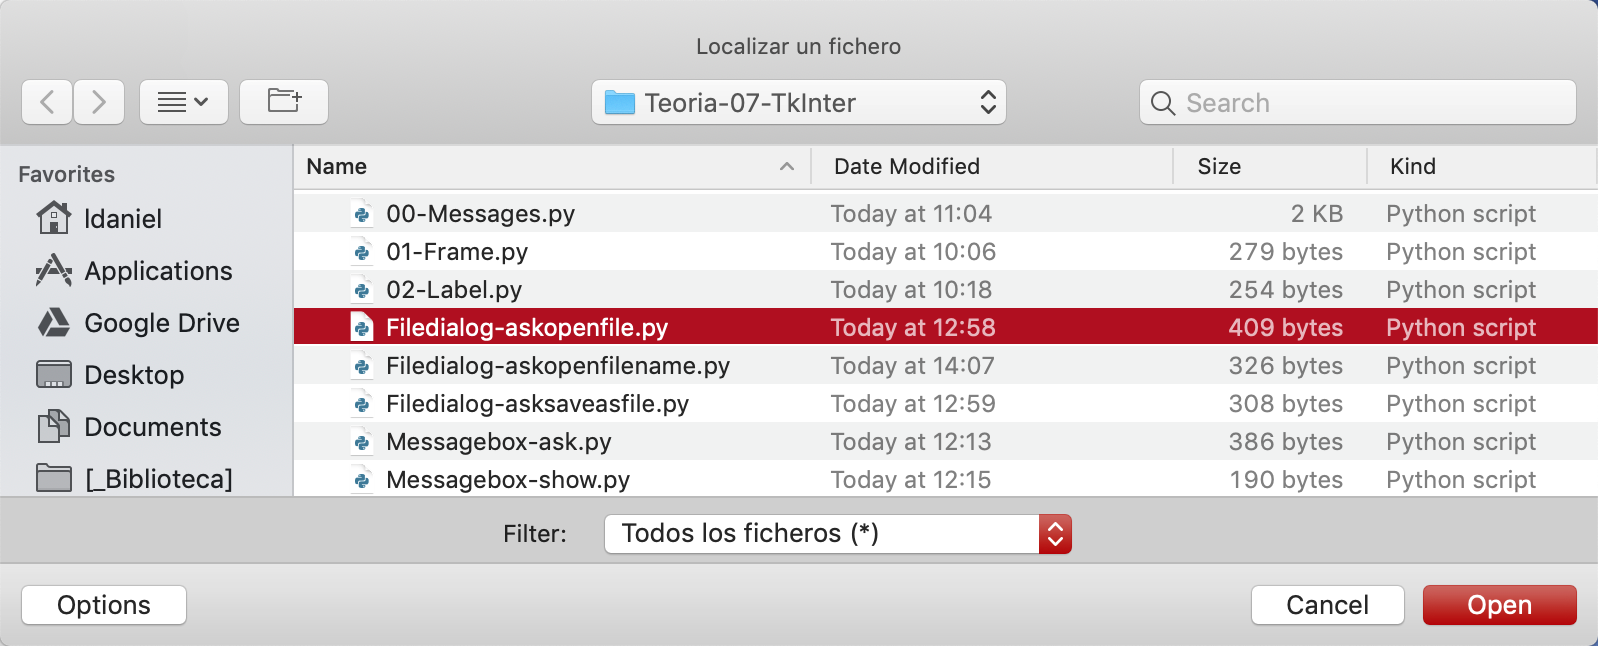
\includegraphics[width=.65\textwidth]{fig/askopenfilename} }

\end{frame}


%%%%%%%%%%%%%%%%%%%%%%%%%%%%%%%%%%%%%
%%%%%%%%%%%%%%%%%%%%%%%%%%%%%%%%%%%%%
\begin{frame}[fragile]{filedialog para Abrir un  Fichero} 
\footnotesize
\begin{pyverbatim}[][frame=single]
from tkinter import filedialog

fichero = filedialog.askopenfile(mode="r",
    initialdir=".",
    filetypes=(("Ficheros de texto", "*.txt"), ("Todos los ficheros", "*.*")),
    title="Leer un fichero"
)

lineas = "Nada que leer"
if fichero is not None:
    lineas = fichero.readlines()
    fichero.close()

print(lineas)

\end{pyverbatim}

\centerline{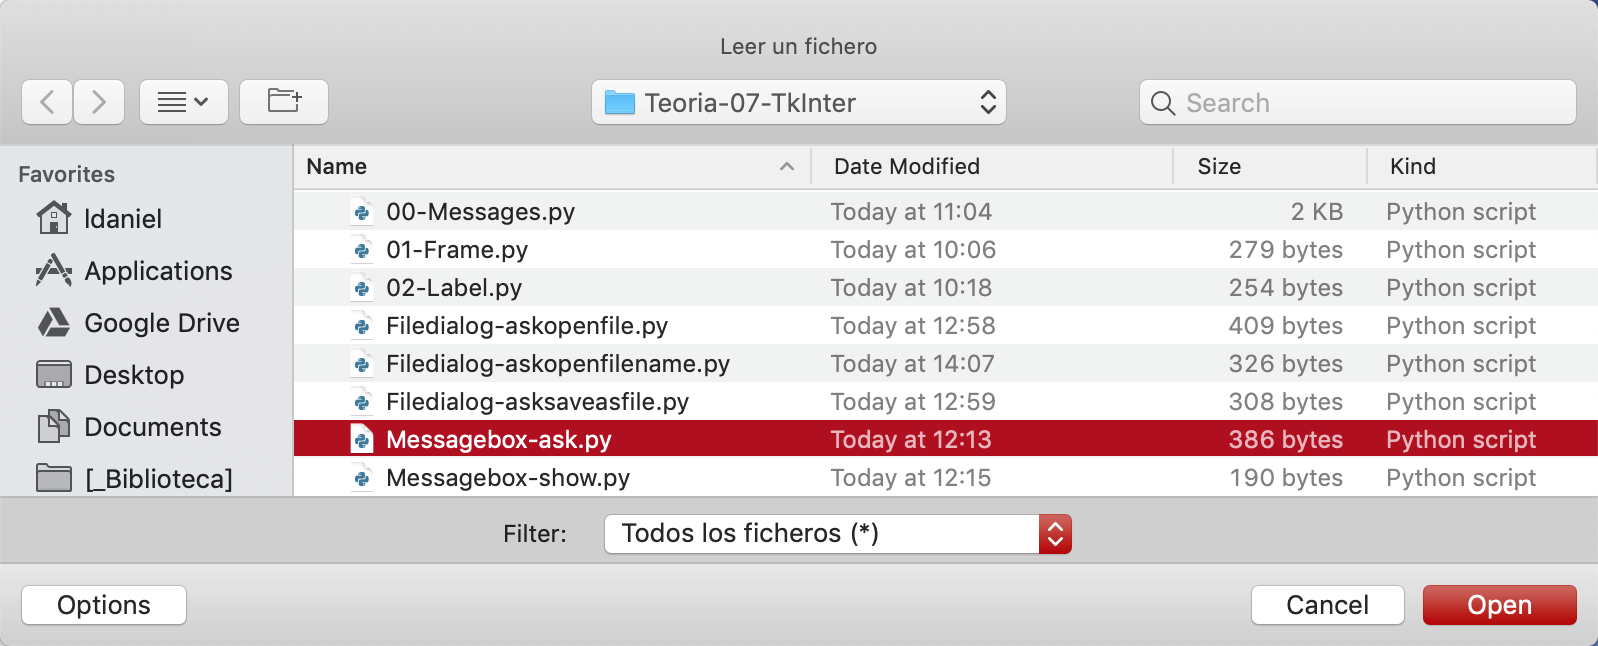
\includegraphics[width=.65\textwidth]{fig/askopenfile} }

\end{frame}




%%%%%%%%%%%%%%%%%%%%%%%%%%%%%%%%%%%%%
%%%%%%%%%%%%%%%%%%%%%%%%%%%%%%%%%%%%%
\begin{frame}[fragile]{filedialog para Escribir un  Fichero} 
\footnotesize
\begin{pyverbatim}[][frame=single]
from tkinter import filedialog

fichero = filedialog.askopenfile(mode="w",
    initialdir=".",
    title="Guardar en un fichero"
)

lineas = ["Un par\n", "de lineas\n"]
if fichero is not None:
    fichero.writelines(lineas)
    fichero.close()

\end{pyverbatim}

\centerline{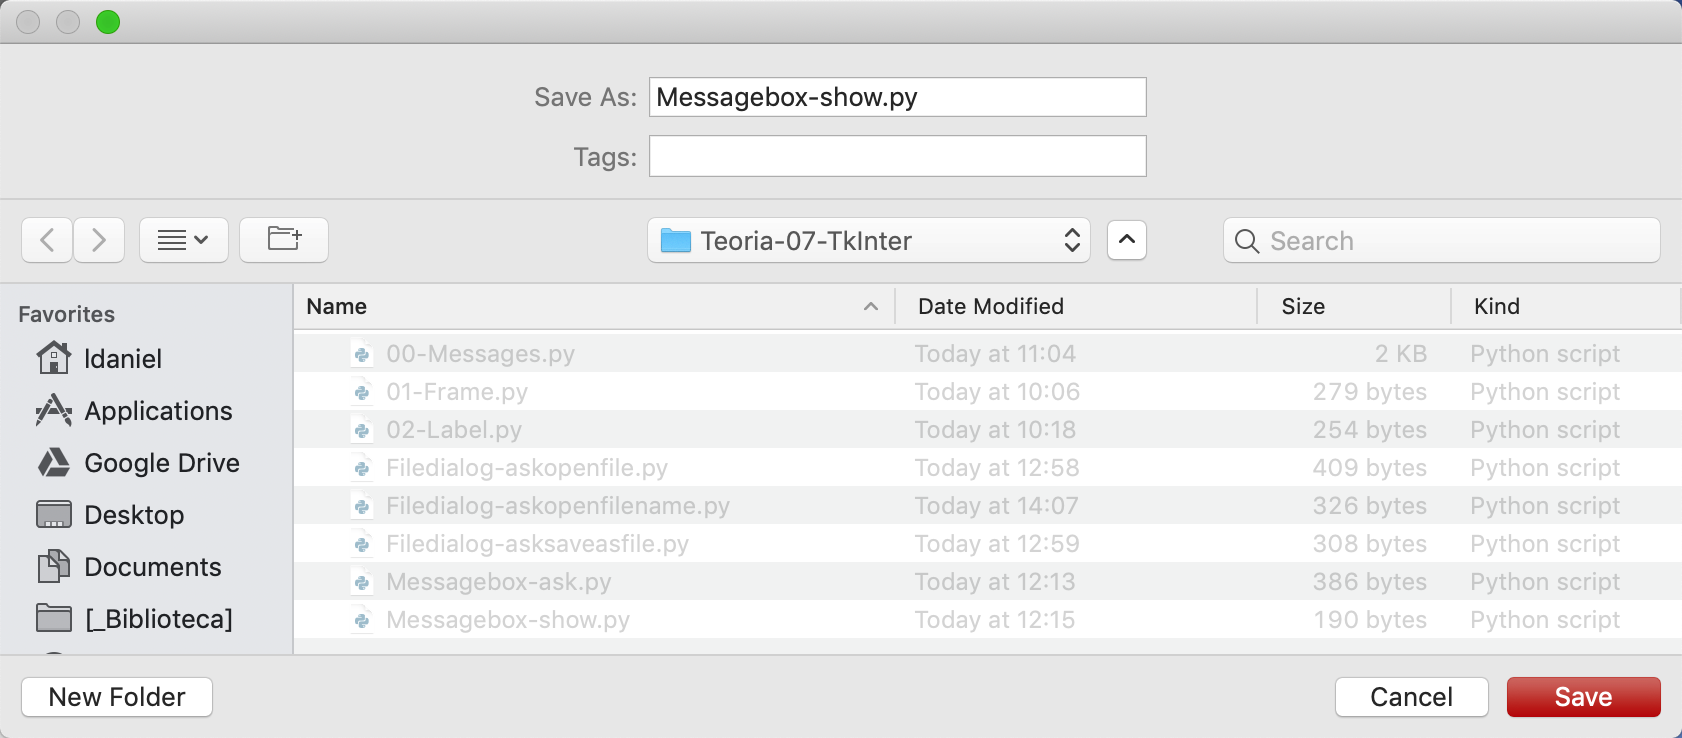
\includegraphics[width=.65\textwidth]{fig/asksaveasfile} }

\end{frame}




%%%%%%%%%%%%%%%%%%%%%%%%%%%%%%%%%%%%%
%%%%%%%%%%%%%%%%%%%%%%%%%%%%%%%%%%%%%
\subsection{tkinter.simpledialog}



%%%%%%%%%%%%%%%%%%%%%%%%%%%%%%%%%%%%%
%%%%%%%%%%%%%%%%%%%%%%%%%%%%%%%%%%%%%
\begin{frame}[fragile]{Tres formas de pedir datos con \cm{simpledialog}} 

\footnotesize
\begin{pyverbatim}[][frame=single]
import tkinter as tk
from tkinter import simpledialog
window = tk.Tk()  # NO olvides la ventana padre
answer = simpledialog.askstring("Input", "Tu nombre?", parent=window)
answer = simpledialog.askinteger("Input", "Tu edad?",  parent=window,
                                 minvalue=0, maxvalue=100)
answer = simpledialog.askfloat("Input", "Tu sueldo?",  parent=window,
                               minvalue=0.0, maxvalue=100000.0)
\end{pyverbatim}

\begin{itemize}
\item
Si al pedir un dato no cumple las restricciones se mostrará un ventana de aviso.

\unEjemplo Ventanas de aviso al pedir un entero

\hfil\begin{minipage}{.8\textwidth}
\centerline{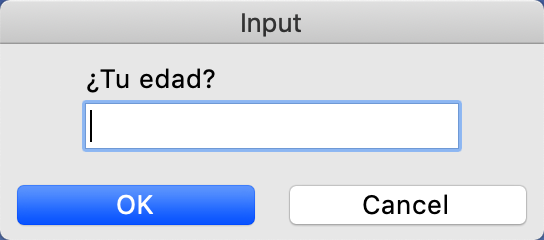
\includegraphics[width=.4\textwidth]{fig/askinteger} \hfill
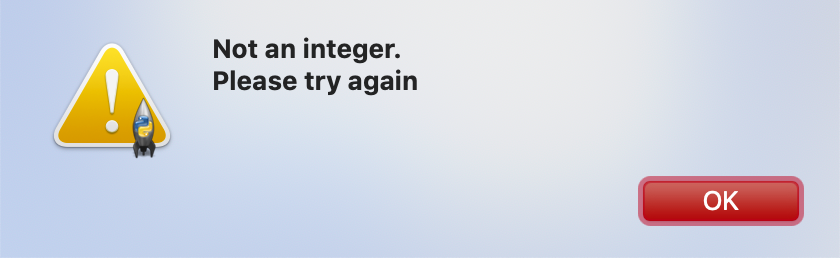
\includegraphics[width=.45\textwidth]{fig/askintegerError}
}

\centerline{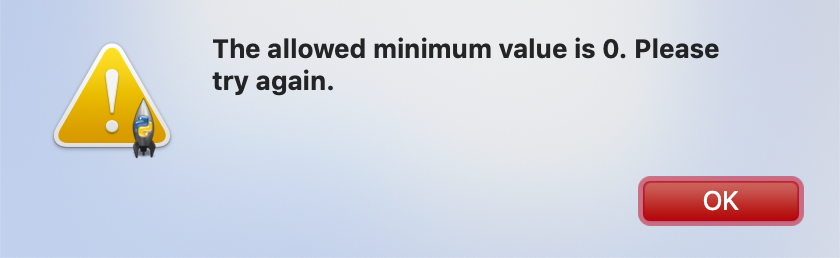
\includegraphics[width=.45\textwidth]{fig/askintegerMin} \hfill
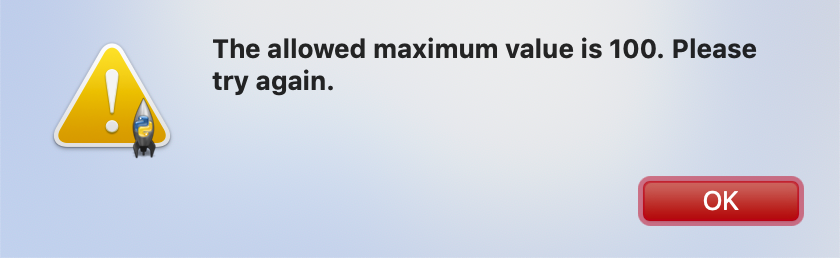
\includegraphics[width=.45\textwidth]{fig/askintegerMax}
}
\end{minipage}
\end{itemize}


\end{frame}






%%%%%%%%%%%%%%%%%%%%%%%%%%%%%%%%%%%%%
%%%%%%%%%%%%%%%%%%%%%%%%%%%%%%%%%%%%%
\begin{frame}{Ejercicio} 

\begin{ejercicio}{}
Construye un programa que haga lo siguiente, en este orden:

\begin{enumerate}
\item Solicita el nombre y edad de dos personas.

\begin{itemize}
\item La longitud del nombre no puede ser vacío y tienen que ser al menos de 3  caracteres. \item La edad mínima será 16.
\item La información de cada persona es una tupla.
\end{itemize}

\item Guarda la información en un fichero.

\begin{itemize}
\item Pide al usuario que te indique el nombre del fichero.
\item Los datos de cada persona ocupan una línea.
\end{itemize}

\item Muestra un mensaje informativo de que toda la tarea se ha realizado.
\end{enumerate}

\end{ejercicio}



\end{frame}






%%%%%%%%%%%%%%%%%%%%%%%%%%%%%%%%%%%%%
%%%%%%%%%%%%%%%%%%%%%%%%%%%%%%%%%%%%%

\section{Construcción de Interface Gráficas de Usuario}

%%%%%%%%%%%%%%%%%%%%%%%%%%%%%%%%%%%%%
%%%%%%%%%%%%%%%%%%%%%%%%%%%%%%%%%%%%%
\begin{frame}{Widgets}
\begin{itemize}
\item Widgets Básicos:
	\begin{itemize}
	\item Frame: Contenedor de widgets
	\item Label: Etiquetas (de texto o gráfica)
	\item Buttom: Botón
	\item Checkbutton: Seleccionar o no una opción. Pueden ser varias.
	\item Radiobutton:  Seleccionar una opción. 
	\item Entry: Introducir un texto
	\end{itemize}
	
\item Otros widgets (hay más):
	\begin{itemize}
	\item Listbox: Seleccionar una o varias entradas de una lista de opciones.
	\item Combobox: Seleccionar una entrada de una lista de opciones.
	\item Text: Introducir varias líneas de texto.
	\item Scrollbar: Barra de desplazamiento cuando el contenido es demasiado grande.
	\item Scale: Barra de desplazamiento para seleccionar un valor numéricos.
	\item Spinbox: Seleccionar un número (o de  una lista arbitraria) con flecha arriba/abajo.
	\item Progressbar: Da al usuario feedback del progreso de la operación.
	\item Canvas: Dibuja líneas, círculos, texto, imágenes, ...
	\item Treeview: Muestra una jerarquía de items y permite que el usuario los visualice.
	\item Separator: Muestra una línea de separación.
	\item Notebook: Pestañas
	\end{itemize}

\item Objetos que no son widgets: menús, ventanas (de diálogo, de directorios, de ficheros, de colores).

\end{itemize}
\end{frame}



%%%%%%%%%%%%%%%%%%%%%%%%%%%%%%%%%%%%%
%%%%%%%%%%%%%%%%%%%%%%%%%%%%%%%%%%%%%
\subsection{Tk, Frame}

%%%%%%%%%%%%%%%%%%%%%%%%%%%%%%%%%%%%%
%%%%%%%%%%%%%%%%%%%%%%%%%%%%%%%%%%%%%
\begin{frame}[fragile]{Creación de Ventanas: \cm{Tk()}}

\begin{itemize}
\item El sistema de coordenadas considera el origen (0, 0) en la esquina superior izquierda.
\item Sobre una ventana se debe de crear uno o varios Frames (widget).
\item Sobre cada Frame se colocarán otros widgets (botones, etiquetas, ...)
\end{itemize}

\footnotesize
\begin{pyverbatim}[][frame=single]
import tkinter as tk

# Crea Ventana Principal
root = tk.Tk()

# Asigna un título
root.title("Probando Tk")

# Se pueden retocar parámetros en su configuración
root.config(bg="Aqua")

# Ejecución de un bucle sin fin con eventos
root.mainloop()
\end{pyverbatim}

\begin{textblock*}{.4\textwidth}(.6\textwidth,0.42\textheight)
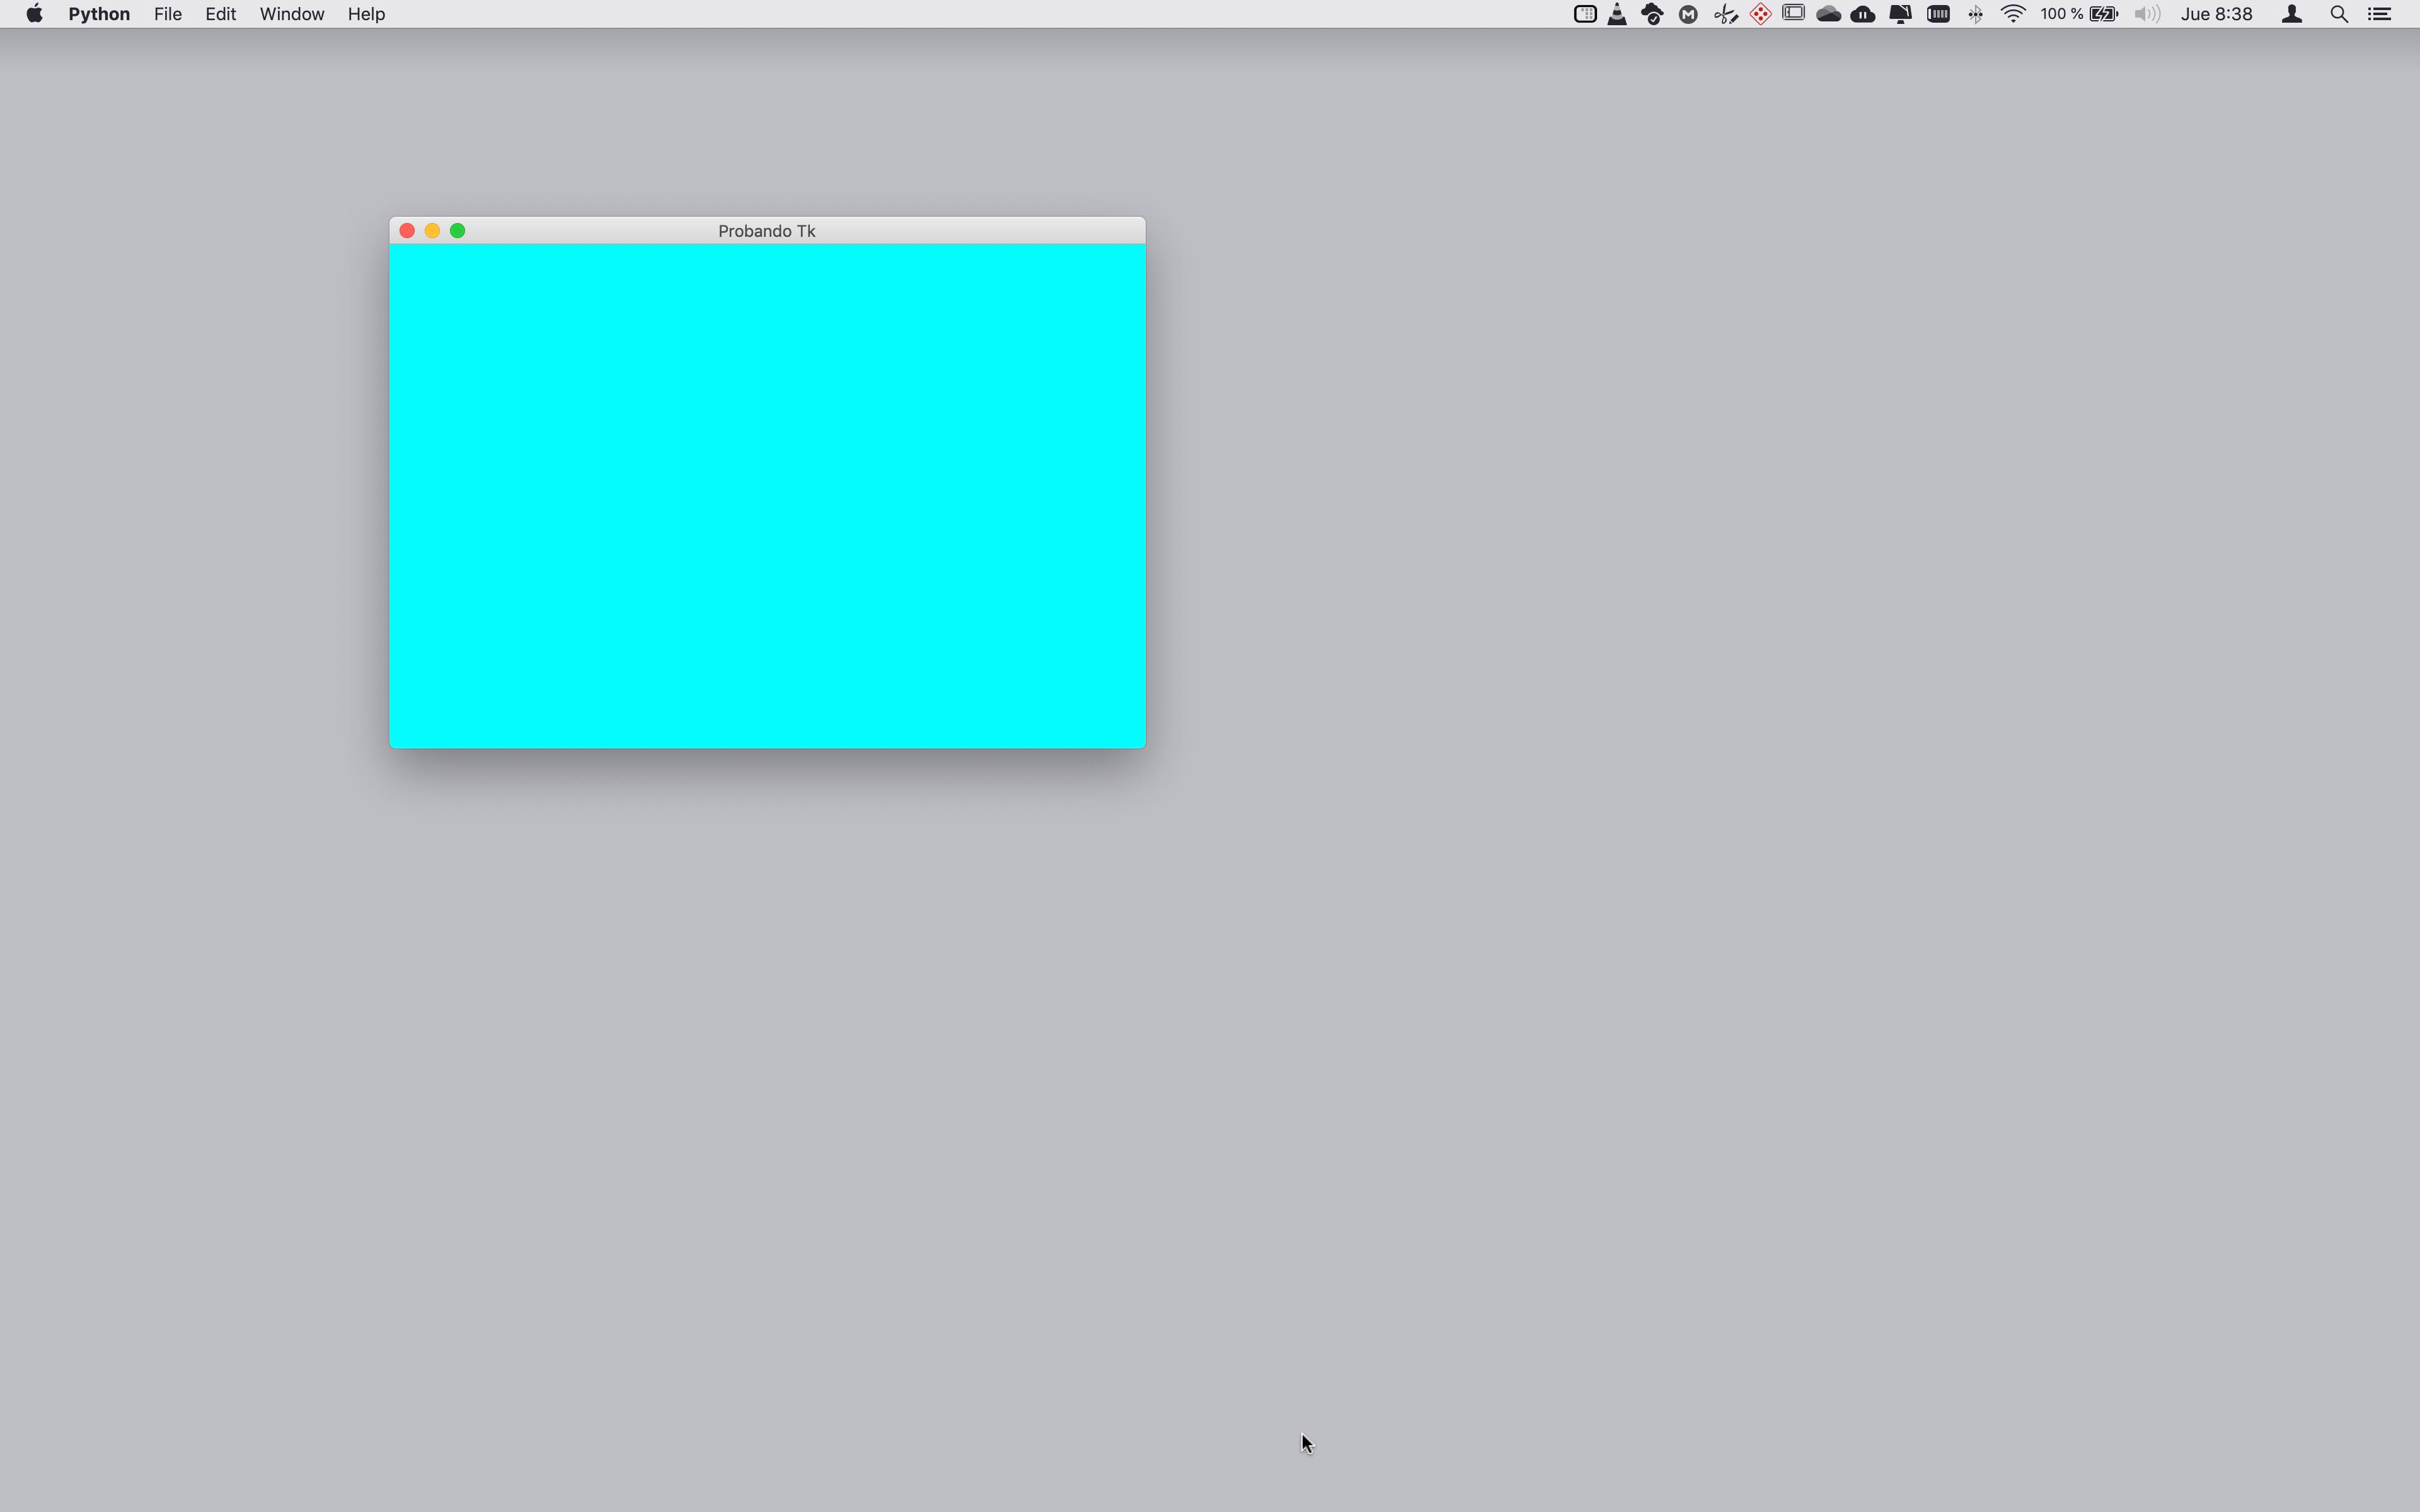
\includegraphics[width=\textwidth]{fig/tk}
\end{textblock*}


\end{frame}




%%%%%%%%%%%%%%%%%%%%%%%%%%%%%%%%%%%%%
%%%%%%%%%%%%%%%%%%%%%%%%%%%%%%%%%%%%%
\begin{frame}[fragile]{Widgets Básicos: Frame}
{\pyv{frame = tk.Frame(root)}}

\begin{pyverbatim}[][frame=single]
import tkinter as tk

root = tk.Tk()
root.geometry("720x350")

frame = tk.Frame(root)
frame.config(width="350", height="200")
frame.config(borderwidth='10', relief='groove')
frame.config(bg="red")

frame.pack(side="right")  # 'left', 'right', 'top', 'bottom'

root.mainloop()
\end{pyverbatim}

\begin{textblock*}{.4\textwidth}(.6\textwidth,0.21\textheight)
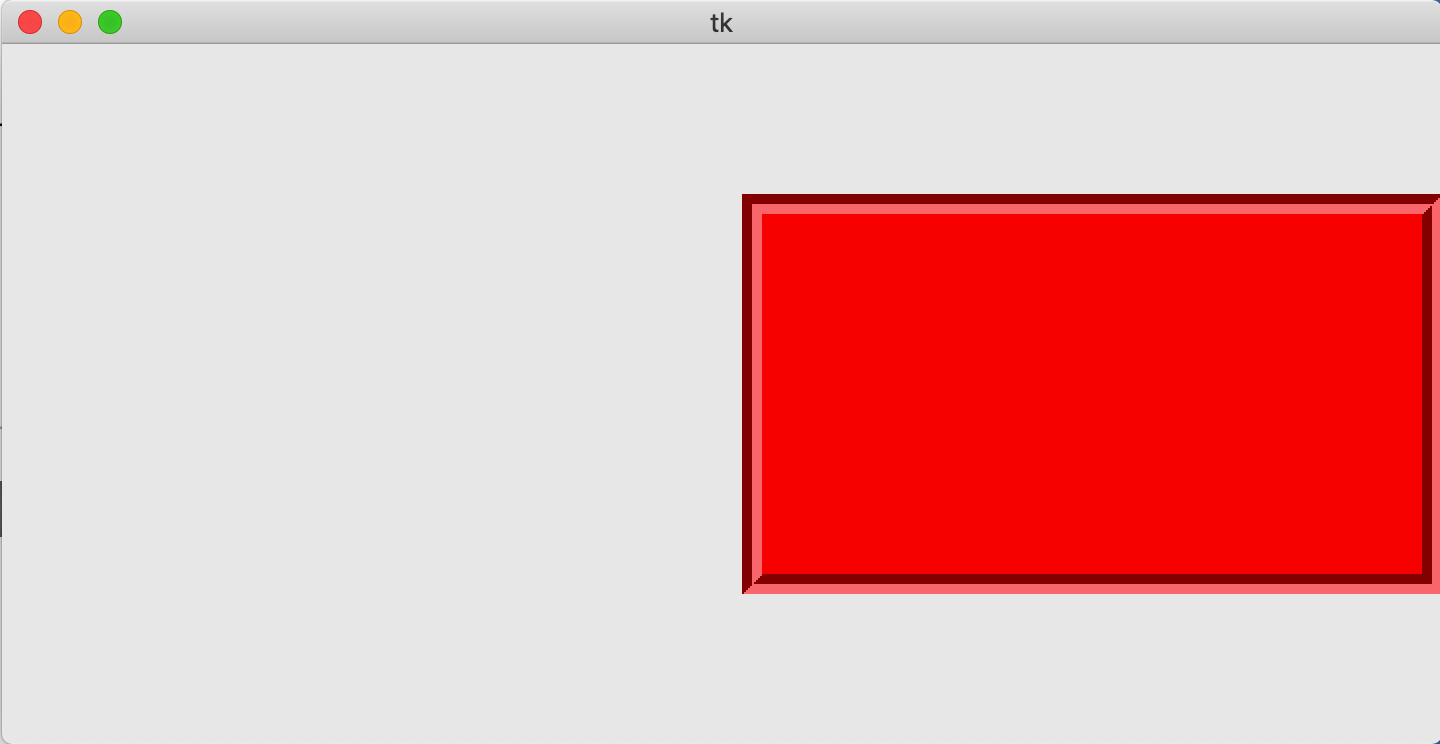
\includegraphics[width=\textwidth]{fig/FrameScreen}
\end{textblock*}

\:


\centerline{Relief: 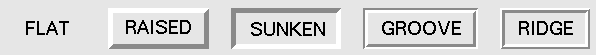
\includegraphics[width=.45\textwidth]{fig/relief.png}}

\vfill

{\scriptsize $\bullet$
Para \cm{pack()} ver pág. \pageref{pack}.
}
\end{frame}




%%%%%%%%%%%%%%%%%%%%%%%%%%%%%%%%%%%%%
%%%%%%%%%%%%%%%%%%%%%%%%%%%%%%%%%%%%%
\subsection{Label}



%%%%%%%%%%%%%%%%%%%%%%%%%%%%%%%%%%%%%
%%%%%%%%%%%%%%%%%%%%%%%%%%%%%%%%%%%%%
\begin{frame}[fragile]{Widgets Básicos: Label}
{\pyv{label = tk.Label(frame, text="txt")} con {\tt place()}}

\begin{pyverbatim}[][frame=single]
root = tk.Tk()
root.title("Probando Label")


frame = tk.Frame(root, width=350, 
                                      height=200)
frame.pack()


label = tk.Label(frame, text="Esto es una prueba")
label.place(x=50, y=100)
label.config(fg="yellow", bg="blue")
label.config(font=("Verdana", 24))


root.mainloop()
\end{pyverbatim}

\begin{textblock*}{.25\textwidth}(.7\textwidth,0.2\textheight)
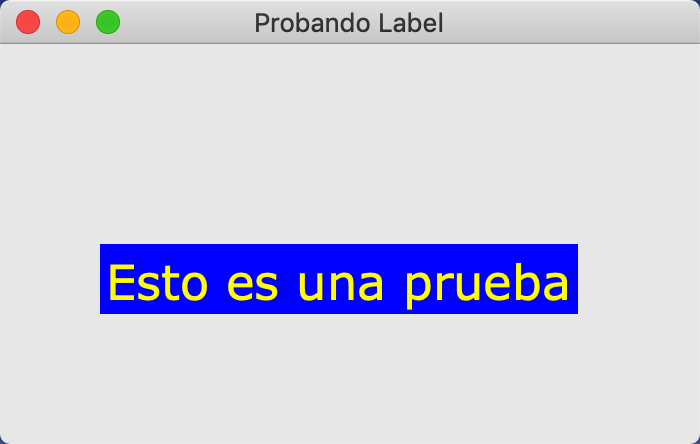
\includegraphics[width=\textwidth]{fig/label-sin-pack}
\end{textblock*}

{\scriptsize $\bullet$
Para \cm{place()} ver pág. \pageref{place}.
}
\end{frame}




%%%%%%%%%%%%%%%%%%%%%%%%%%%%%%%%%%%%%
%%%%%%%%%%%%%%%%%%%%%%%%%%%%%%%%%%%%%
\begin{frame}[fragile]{Widgets Básicos: Label}
{\pyv{label = tk.Label(frame, text="txt")} con {\tt pack()}}

\begin{pyverbatim}[][frame=single]
root = tk.Tk()
root.title("Probando Label")


frame = tk.Frame(root)
frame.pack()

tk.Label(frame, text="!Hola Mundo!").pack(anchor='nw')
tk.Label(frame, text="!Otra etiqueta muy muy larga!").
                                         pack(anchor='center')
tk.Label(frame, text="!Última etiqueta!").pack(anchor='se')

root.mainloop()
\end{pyverbatim}

\begin{textblock*}{.4\textwidth}(.7\textwidth,0.2\textheight)
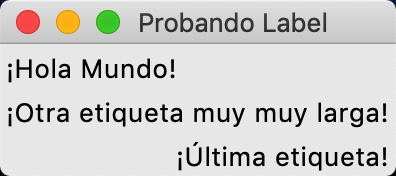
\includegraphics[width=\textwidth]{fig/label-con-pack}
\end{textblock*}

{\scriptsize $\bullet$
Para \cm{pack()} ver pág. \pageref{pack}.
}
\end{frame}




%%%%%%%%%%%%%%%%%%%%%%%%%%%%%%%%%%%%%
%%%%%%%%%%%%%%%%%%%%%%%%%%%%%%%%%%%%%
\begin{frame}[fragile]{Widgets Básicos: Label}
{\pyv{label = tk.Label(frame, img=un_imagen)}}

\begin{pyverbatim}[][frame=single]
root = tk.Tk()
root.title("Probando Label con Imagen")
root.geometry("350x200+100+100")


frame = tk.Frame(root, width=350, height=200)
frame.pack()

mi_imagen=tk.PhotoImage(file="./ldaniel.png")

label = tk.Label(frame, image=mi_imagen)
label.place(x=50, y=40)

root.mainloop()
\end{pyverbatim}

\begin{textblock*}{.3\textwidth}(.8\textwidth,0.2\textheight)
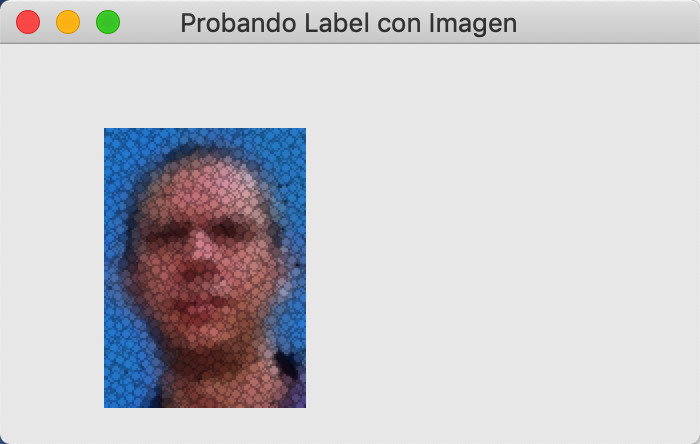
\includegraphics[width=\textwidth]{fig/label-con-imagen}
\end{textblock*}


{\scriptsize $\bullet$
Para \cm{place()} ver pág. \pageref{place}.
}
\end{frame}




%%%%%%%%%%%%%%%%%%%%%%%%%%%%%%%%%%%%%
%%%%%%%%%%%%%%%%%%%%%%%%%%%%%%%%%%%%%
\begin{frame}[fragile]{Label con un StringVar cualquiera}
\small
\begin{pyverbatim}[][frame=single]
root = tk.Tk()
contador = 0
root.title("Label con StringVar")
frame = tk.Frame(root, width=150, height=100).pack()
label = tk.Label(frame).place(x=50, y=25)
label.config(font=("Verdana", 24))
    
# El StringVar es un objeto libre
string_var = StringVar(value="Mensaje Inicial")

while True:
    contador += 1
    root.update_idletasks()
    root.update()
    time.sleep(0.1)
    # ESTO ES LO IMPORTANTE
    string_var.set(str(contador))
    # ^^^^^ En cada iteración se asigna nuevo valor a string_var
    label.config(text=string_var.get())  # <<<<
    # ^^^^^ En cada iteración reconfiguro Label
\end{pyverbatim}

\begin{textblock*}{.25\textwidth}(.7\textwidth,.6\textheight)
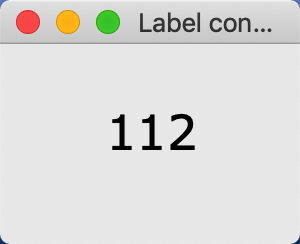
\includegraphics[width=\textwidth]{fig/label-stringvar}
\end{textblock*}

\end{frame}



%%%%%%%%%%%%%%%%%%%%%%%%%%%%%%%%%%%%%
%%%%%%%%%%%%%%%%%%%%%%%%%%%%%%%%%%%%%
\begin{frame}[fragile]{Vinculando un Label a un StringVar: \cm{textvariable}}
\small
\begin{pyverbatim}[][frame=single]
contador=0
root = tk.Tk()
root.title("Label con StringVar")
frame = tk.Frame(root, width=150, height=100).pack()

# Vinculamos el StringVar al Label
string_var=StringVar(value="Mensaje Inicial")
label = tk.Label(frame, textvariable=string_var) # <<<< Vinculación
label.place(x=50, y=25)
label.config(font=("Verdana", 24))

while True:
    contador += 1
    root.update_idletasks()
    root.update()
    time.sleep(0.1)
    # Basta cambiar string_var para que cambie Label
    string_var.set(str(contador))
    # ^^^^^ En cada iteración se asigna nuevo valor a string_var
    #       No se necesita reconfigurar Label
\end{pyverbatim}

\begin{textblock*}{.25\textwidth}(.7\textwidth,0.5\textheight)
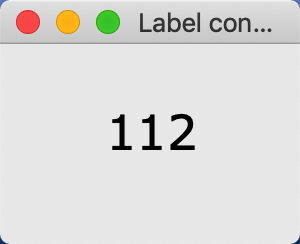
\includegraphics[width=\textwidth]{fig/label-stringvar}
\end{textblock*}

\end{frame}






%%%%%%%%%%%%%%%%%%%%%%%%%%%%%%%%%%%%%
%%%%%%%%%%%%%%%%%%%%%%%%%%%%%%%%%%%%%
\subsection{Entry, Text}

%%%%%%%%%%%%%%%%%%%%%%%%%%%%%%%%%%%%%
%%%%%%%%%%%%%%%%%%%%%%%%%%%%%%%%%%%%%
\begin{frame}[fragile]{Widgets Básicos: Entry  (texto corto)}
{\pyv{entry = tk.Entry(frame)}}

\begin{pyverbatim}[][frame=single]
import tkinter as tk

root = tk.Tk()
root.title("Probando Entry")

frame = tk.Frame(root, width=350, height=200)
frame.pack()

tk.Label(frame, text="Escribe algo:").pack(padx=10)


tk.Entry(frame).pack(padx=100, pady=30, ipadx=50, ipady=5)


root.mainloop()
\end{pyverbatim}

\begin{textblock*}{.5\textwidth}(.5\textwidth,0.15\textheight)
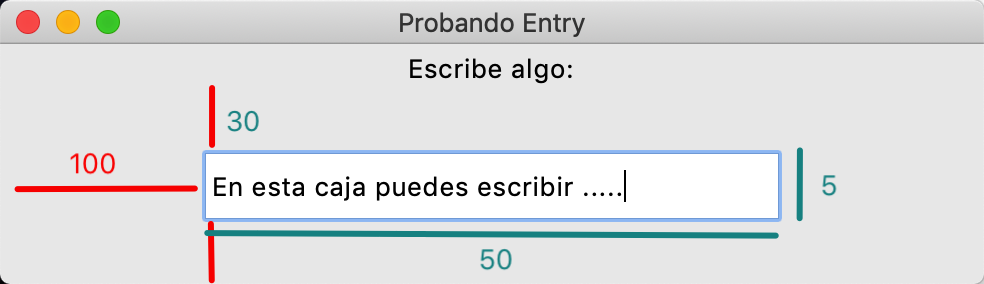
\includegraphics[width=\textwidth]{fig/entry}
\end{textblock*}


{\scriptsize $\bullet$
Para \cm{pack()} ver pág. \pageref{pack}.
}
\end{frame}



%%%%%%%%%%%%%%%%%%%%%%%%%%%%%%%%%%%%%
%%%%%%%%%%%%%%%%%%%%%%%%%%%%%%%%%%%%%
\begin{frame}[fragile]{Widgets Básicos: Text  (texto largo)}
{\pyv{text = tk.Text(frame)}}

\begin{pyverbatim}[][frame=single]
import tkinter as tk

root = tk.Tk()
root.title("Probando Entry")
frame = tk.Frame(root, 
             width=350, 
             height=200)
frame.pack()


tk.Label(frame, text="Escribe algo:").pack()

text = tk.Text(frame)
text.config(width=30, height=10, font=("Arial", 24))
text.pack(padx=100, pady=30)

root.mainloop()
\end{pyverbatim}

\begin{textblock*}{.5\textwidth}(.6\textwidth,0.15\textheight)
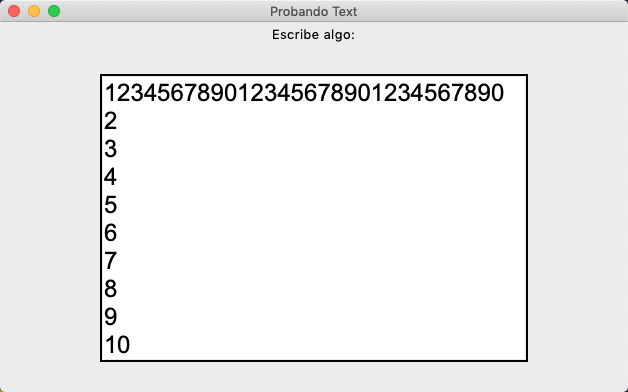
\includegraphics[width=\textwidth]{fig/text}
\end{textblock*}

{\scriptsize $\bullet$
Para \cm{pack()} ver pág. \pageref{pack}.
}
\end{frame}





%%%%%%%%%%%%%%%%%%%%%%%%%%%%%%%%%%%%%
%%%%%%%%%%%%%%%%%%%%%%%%%%%%%%%%%%%%%
\begin{frame}[fragile]{?`Cómo deshabilitar la edición?}
\begin{itemize}
\item Si alguna vez quisiera deshabilitar que se modifique una entrada puede usar alguna de estas opciones.

\item Cambiando el estado de habilitación/deshabilitación.
\begin{pyverbatim}[][frame=single]
text = Text(app, state='disabled', width=44, height=5)
text.configure(state='normal')
text.insert('end', 'Some Text')
text.configure(state='disabled') # Deshabilita el widget
\end{pyverbatim}

\item Indicando que el estado es de solo lectura.
\begin{pyverbatim}[][frame=single]
entry = Entry(frame)
entry.config(state='readonly')) # Habilitado pero no editable
\end{pyverbatim}


\item Vincular cualquier pulsación de tecla a una función que devuelva  ``break'':
\begin{pyverbatim}[][frame=single]
text = Text(app, state='normal', width=44, height=5)
text = Tkinter.Text(root)
text.bind("<Key>", lambda e: "break")
\end{pyverbatim}
\end{itemize}
\end{frame}







%%%%%%%%%%%%%%%%%%%%%%%%%%%%%%%%%%%%%
%%%%%%%%%%%%%%%%%%%%%%%%%%%%%%%%%%%%%
\begin{frame}[fragile]{Entry con StringVar}
\small
\begin{pyverbatim}[][frame=single]
root = tk.Tk()
root.title("Entry con StringVar")
frame = tk.Frame(root, width=150, height=100)
frame.pack()

# Vinculamos el StringVar al Entry
string_var = StringVar(value="Mensaje Inicial")
tk.Entry(frame, textvariable=string_var).pack()

n1 = simpledialog.askfloat("Entrada", 
                           "1er. Número?",
                            parent=root)
n2 = simpledialog.askfloat("Entrada", 
                           "2o. Número?", 
                           parent=root)

#Se cambia el valor del string_var
string_var.set(str(n1+n2))      # Muestra el resultado
entry.config(state='readonly')  # y no se puede modificar
root.mainloop()
\end{pyverbatim}

\begin{textblock*}{.30\textwidth}(.8\textwidth,0.1\textheight)
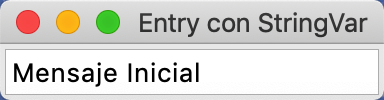
\includegraphics[width=\textwidth]{fig/entry-stringvar1}\\
\; \\
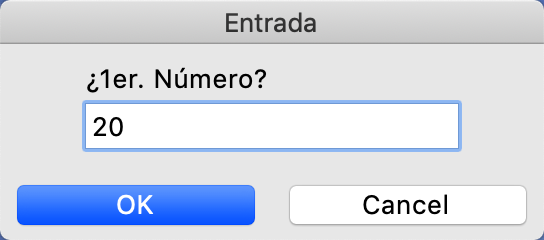
\includegraphics[width=\textwidth]{fig/entry-stringvar2}\\
\; \\
\; \\
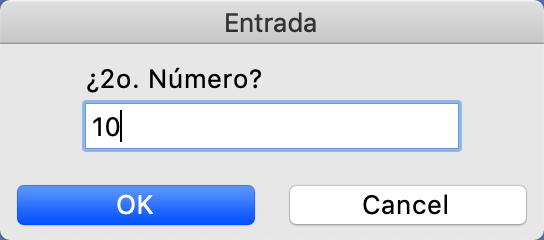
\includegraphics[width=\textwidth]{fig/entry-stringvar3}\\
\; \\
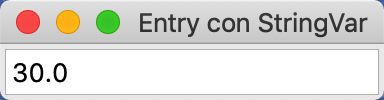
\includegraphics[width=\textwidth]{fig/entry-stringvar4}
\end{textblock*}

\end{frame}





%%%%%%%%%%%%%%%%%%%%%%%%%%%%%%%%%%%%%
%%%%%%%%%%%%%%%%%%%%%%%%%%%%%%%%%%%%%
\subsection{Widgets con Eventos: Button, Radiobutton, Checkbutton}


%%%%%%%%%%%%%%%%%%%%%%%%%%%%%%%%%%%%%
%%%%%%%%%%%%%%%%%%%%%%%%%%%%%%%%%%%%%
\begin{frame}{Eventos}

\begin{itemize}
\item Una aplicación Tkinter pasa la mayor parte de su tiempo dentro de un \key{bucle de eventos} (ingresado a través del método mainloop). 
\item Ejemplos de eventos: pulsar una tecla, mover el ratón, dibujar en el canvas, ...
\item Tkinter permite que \key{a cada widget, se le pueda vincular funciones} y métodos de Python a eventos.

\item \pyv{widget.bind (evento, controlador)}: Si ocurre un evento que coincide con la descripción del evento en el widget, se llama al controlador dado con un objeto que describe el evento.

\unEjemplo \pyv{frame.bind("<Button-1>", callback)} indica que la hacer click con el ratón se invocará a la función \cm{callback()}.

\item Estos son algunos nombres de los eventos: \cm{<Button-1>}, \cm{<ButtonPress-1>}, \cm{<B1-Motion>}, \cm{<ButtonRelease-1>}, \cm{<Enter>}, \cm{<Return>}, \cm{<Key>}, etc ... \\
Puede consultar los siguientes enlaces para su significado: 
	\begin{itemize}\itemsep0pt \tiny
	\item \url{https://effbot.org/tkinterbook/tkinter-events-and-bindings.htm}
	\item \url{http://infohost.nmt.edu/tcc/help/pubs/tkinter/web/event-types.html}
	\item \url{https://www.python-course.eu/tkinter_events_binds.php}
	\end{itemize}
	
	
\item Algunos widget presenta \cm{command} entre sus opciones \key{para indicar la función o método que será invocado} cuando se produzca ciertos eventos:
	\begin{itemize}
	\item Para Button, cuando el widget es \key{pulsado}. 
	\item Para Checkbutton y Radiobutton, cuando el widget \key{cambia su estado}. 
	\end{itemize}
\end{itemize}
\end{frame}







%%%%%%%%%%%%%%%%%%%%%%%%%%%%%%%%%%%%%
%%%%%%%%%%%%%%%%%%%%%%%%%%%%%%%%%%%%%
\begin{frame}[fragile]{Widgets Básicos: Button}
{\pyv{bt = tk.Button(parent, text="txt", command=funcion)}}

\begin{pyverbatim}[][frame=single]
import tkinter as tk

def actua():
    global root
    root.destroy()

root = tk.Tk()
root.title("Probando Buttom")

frame = tk.Frame(root, width=350, height=200)
frame.pack()

button = tk.Button(frame, text='Clícame', command=actua)
button.pack(padx=50, pady=50)

root.mainloop()
\end{pyverbatim}

\begin{textblock*}{.25\textwidth}(.7\textwidth,0.15\textheight)
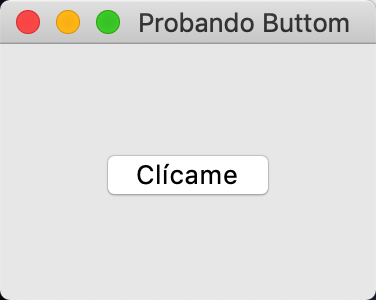
\includegraphics[width=\textwidth]{fig/buttom}
\end{textblock*}

\begin{itemize}
\item Al pulsar el botón se invocará al método \cm{root.destroy()}, el cual terminará la aplicación.
\end{itemize}

\end{frame}



%%%%%%%%%%%%%%%%%%%%%%%%%%%%%%%%%%%%%
%%%%%%%%%%%%%%%%%%%%%%%%%%%%%%%%%%%%%
\begin{frame}[fragile]{Widgets Básicos: Radiobutton}
{\pyv{bt = tk.Radiobutton(parent, text="txt", variable=var, value=v, command=func)}}

\small
\begin{pyverbatim}[][frame=single]
import tkinter as tk
from tkinter import IntVar

def selec():
    t = f"Selección: {opcion.get()}"
    monitor.config(text = t )

root = tk.Tk()
root.config(bd=15)

opcion = IntVar() # Como StrinVar pero en entero

tk.Radiobutton(root, text="Opción 1", variable=opcion,
            value=1, command=selec).pack()
tk.Radiobutton(root, text="Opción 2", variable=opcion,
            value=2, command=selec).pack()

salida = tk.Label(root)
salida.pack()
root.mainloop()
\end{pyverbatim}
{\tiny Fuente: \url{https://docs.hektorprofe.net/python/interfaces-graficas-con-tkinter/widget-radiobutton-radial/}}

\begin{textblock*}{.25\textwidth}(.7\textwidth,0.15\textheight)
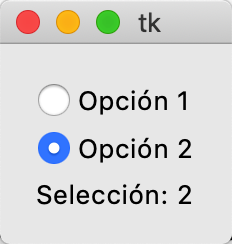
\includegraphics[width=\textwidth]{fig/Radiobutton}
\end{textblock*}

\end{frame}





%%%%%%%%%%%%%%%%%%%%%%%%%%%%%%%%%%%%%
%%%%%%%%%%%%%%%%%%%%%%%%%%%%%%%%%%%%%
\begin{frame}[fragile]{Widgets Básicos: Radiobutton}

\small
\begin{pyverbatim}[][frame=single]
import tkinter as tk
from tkinter import StringVar

def muestraMedida():
    print(sistemaMedida.get())

root = tk.Tk()
root.title("Checkbutton")
root.config(bd=20)

sistemaMedida = StringVar()

tk.Checkbutton(root, text='Sistema Métrico', 
                command=muestraMedida, 
                variable=sistemaMedida,
                onvalue='metrico', 
                offvalue='ingles')
                .pack()
tk.mainloop()
\end{pyverbatim}



\begin{textblock*}{.30\textwidth}(.8\textwidth,0.2\textheight)
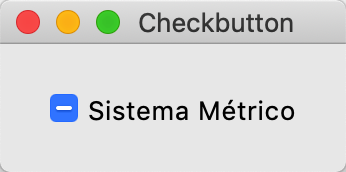
\includegraphics[width=\textwidth]{fig/Checkbutton1}\\
\; \\
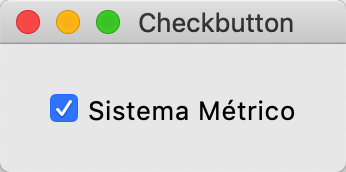
\includegraphics[width=\textwidth]{fig/Checkbutton2}\\
\; \\
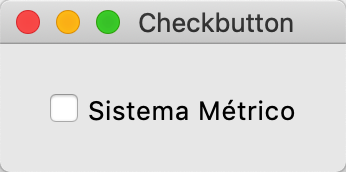
\includegraphics[width=\textwidth]{fig/Checkbutton3}
\end{textblock*}
\end{frame}






%%%%%%%%%%%%%%%%%%%%%%%%%%%%%%%%%%%%%
%%%%%%%%%%%%%%%%%%%%%%%%%%%%%%%%%%%%%
\subsection{Gráficos: Canvas}



%%%%%%%%%%%%%%%%%%%%%%%%%%%%%%%%%%%%%
%%%%%%%%%%%%%%%%%%%%%%%%%%%%%%%%%%%%%
\begin{frame}[fragile]{Canvas}
{\pyv{canvas = tk.Canvas(parent, width= , height= , bg= )}} 
\begin{itemize}
\item El widget Canvas proporciona una superficie sobre la que se puede dibujar, mostrar imágenes, texto, etc.
\item El origen de coordenadas se sitúa en la parte superior izquierda.
\item Colocado el canvas en la ventana se usan los métodos \cm{create\_xxx()}.

\begin{itemize}
\item \pyv{canvas.create_rectangle(50, 20, 150, 80, fill="#476042")}
\item \pyv{canvas.create_line(0, 0, 50, 20, fill="#476042", width=3)}
\item \pyv{canvas.create_oval(x0, y0, x1, y1, opciones, ... )}

	\begin{columns}
	\begin{column}{.25\textwidth}
		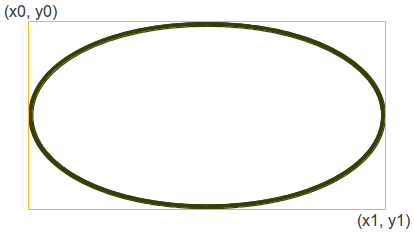
\includegraphics[height=.2\textheight]{fig/canvas_oval}
	\end{column}
	\begin{column}{.65\textwidth}
\begin{pyverbatim}[][frame=single]
def circle(canvas, x, y, r):
   id = canvas.create_oval(x-r,y-r,x+r,y+r)
   return id
\end{pyverbatim}
	\end{column}
	\end{columns}	
	
\item \pyv{canvas.create_text(10, 20, text="Python")}
\item \pyv{canvas.create_image(10, 20, image=img)} donde \pyv{img=PhotImage(file="file.png")}
\item También se puede añadir polígonos. 

Consulte \url{https://python-course.eu/tkinter_canvas.php} si quiere un mini tutorial sobre esto.
\end{itemize}
\end{itemize}

%
%\begin{pyverbatim}[][frame=single]
%root = tk.Tk()
%
%\end{pyverbatim}
%
%\begin{textblock*}{.4\textwidth}(.6\textwidth,0.2\textheight)
%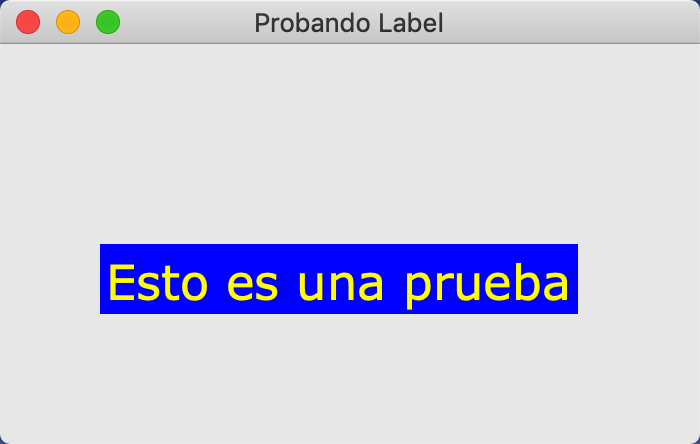
\includegraphics[width=\textwidth]{fig/label-sin-pack}
%\end{textblock*}
%

\end{frame}




%%%%%%%%%%%%%%%%%%%%%%%%%%%%%%%%%%%%%
%%%%%%%%%%%%%%%%%%%%%%%%%%%%%%%%%%%%%
\subsection{Distribución de los Widget en la Ventana}


%%%%%%%%%%%%%%%%%%%%%%%%%%%%%%%%%%%%%
%%%%%%%%%%%%%%%%%%%%%%%%%%%%%%%%%%%%%
\begin{frame}{Métodos de distribución}

\begin{itemize} 
\item Tk provee tres métodos para establecer la posición de los  widgets dentro de una ventana
\item Se corresponden con los métodos \cm{.place()},  \cm{.pack()}  y \cm{.grid()}.
\item  \cm{.place()} ubica el elemento indicando su posición absoluta respecto del padre.
\item  \cm{.pack()} coloca el elemento de forma relativa a los elementos previos.
\item  \cm{.grid()} divide la ventana en filas y columnas formando celdas. Se coloca el elemento en la celda que se indique.
\end{itemize}

\end{frame}


%%%%%%%%%%%%%%%%%%%%%%%%%%%%%%%%%%%%%
%%%%%%%%%%%%%%%%%%%%%%%%%%%%%%%%%%%%%
\begin{frame}{Método \cm{.place()}}

\begin{itemize} 
\item  \cm{.place()} ubica el elemento indicando su posición absoluta respecto del padre.
\item \cm{x=60, y=40} coloca el objeto en la posición (60, 40) respecto del origen.
\item \cm{relx=0.1, rely=0.1} Indica la posición relativa al tamaño de la ventana.
	\begin{itemize}
	\item Toma valores entre 0 y 1.
	\item Si el ancho de la ventana son 300px, \cm{relx=0.1} indica que se colocará en la posición \cm{x=30}=0.1$\times$300.
	\end{itemize}
	
\item \cm{width=100, height=30} Indica el ancho y alto en píxeles del objeto.
\item \cm{relwidth=0.5, relheight=0.5} Indica el tamaño del objeto relativo al tamaño de la ventana. 
	\begin{itemize}
	\item Toma valores entre 0 y 1.
	\item 0.5 indica que será la mitad del tamaño de la ventana.
	\end{itemize}
	
\item Tiene ejemplos de uso en las páginas anteriores.
\end{itemize}

\end{frame}




%%%%%%%%%%%%%%%%%%%%%%%%%%%%%%%%%%%%%
%%%%%%%%%%%%%%%%%%%%%%%%%%%%%%%%%%%%%
\begin{frame}[fragile, label=place]{Método \cm{.place()}}

\small
\begin{pyverbatim}[][frame=single]
import tkinter as tk

root = tk.Tk()
root.geometry("300x100+200+200")
root.title("Label")


button1=tk.Button(root, text="Pos. absoluta")
button1.place(x=10, y = 10, width=290, height=50)

button2=tk.Button(root, text="Pos. realativa")
button2.place(relx=.5, rely=.5, 
                       relwidth=.5, relheight=.5)

tk.mainloop()
\end{pyverbatim}



\begin{textblock*}{.25\textwidth}(.9\textwidth,0.3\textheight)
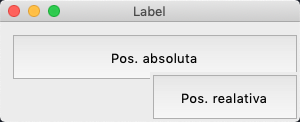
\includegraphics[width=\textwidth]{fig/place1}\\
\; \\
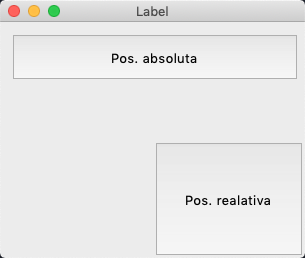
\includegraphics[width=\textwidth]{fig/place2}\\
\; \\
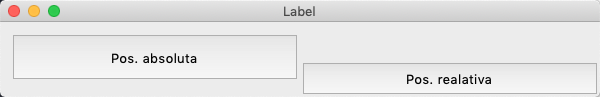
\includegraphics[width=\textwidth]{fig/place3}
\end{textblock*}
\end{frame}




%%%%%%%%%%%%%%%%%%%%%%%%%%%%%%%%%%%%%
%%%%%%%%%%%%%%%%%%%%%%%%%%%%%%%%%%%%%
\begin{frame}[fragile, label=pack]{Método \cm{.pack()}}

\begin{itemize} 
\item  \cm{.pack()} coloca el elemento de forma relativa a los elementos previos.
\item  \cm{.pack()} sin argumentos ubica al elemento debajo del anterior.
\item \cm{side=tk.xxx} coloca el widget en el lado que se indique. 
	\begin{itemize}
	\item Sus valores son: \cm{tk.TOP} (por defecto),\cm{ tk.BOTTOM}, \cm{tk.LEFT}, \cm{tk.RIGHT}.
	\end{itemize}
\item \cm{padx}, \cm{pady} especifican (en píxeles) los márgenes externos de un elemento.
\item \cm{ipadx},  \cm{ipady} que especifican (en píxeles) los márgenes internos de un elemento.

\small
\begin{minipage}{.70\textwidth}
\begin{pyverbatim}[][frame=single]
button = tk.Button(frame, text="Hola, mundo!")
button.pack(padx=30, pady=30, ipadx=50, ipady=50)
\end{pyverbatim}
\end{minipage}
\normalsize

\item Se puede expandir o contraer el elemento a medida que cambie\\
la ventana (\cm{expand=True}), indicando la dirección \\
(\cm{fill=tk.X}, \cm{fill=tk.Y} o \cm{fill=tk.BOTH})

\small
\begin{minipage}{.70\textwidth}
\begin{pyverbatim}[][frame=single]
button.pack(expand=True, fill=tk.BOTH, 
                    padx=10, pady=10)
\end{pyverbatim}
\end{minipage}
\normalsize

\item Tiene ejemplos de uso en las páginas anteriores.

\end{itemize}


\begin{textblock*}{.25\textwidth}(.9\textwidth,0.5\textheight)
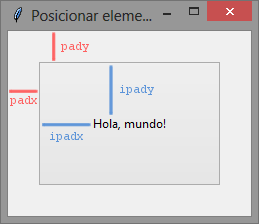
\includegraphics[height=.23\textheight]{fig/padx-pady-ipadx-ipady-tkinter.png}\\
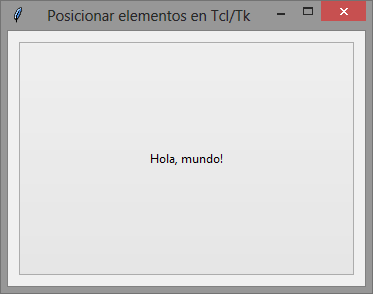
\includegraphics[height=.23\textheight]{fig/elemento-en-expansion-tkinter.png}\\
\end{textblock*}

{\tiny Fuente: \url{https://recursospython.com/guias-y-manuales/posicionar-elementos-en-tkinter/}}
\end{frame}






%%%%%%%%%%%%%%%%%%%%%%%%%%%%%%%%%%%%%
%%%%%%%%%%%%%%%%%%%%%%%%%%%%%%%%%%%%%
\begin{frame}{Método \cm{.grid()}}

\begin{itemize} 
\item \cm{.grid()} divide la ventana en filas y columnas formando celdas.

\item El elemento se coloca en la celda/coordenadas que se indique.

\item Las \key{coordenadas} se especifican con \cm{row=posY}, \cm{column=posX}.

\item Dentro de la celda el elemento \key{se puede posicionar} en una zona concreta con  \cm{sticky="lugar"}.
Las opciones son  \cm{"n"}(norte), \cm{"s"}(sur), \cm{"\/e\/"}(este) o \cm{"w"}(oeste).

\item Si se indican varias posiciones, el widget se expandirá.
\begin{itemize}
\item Ejemplo, \cm{sticky="nsew"} expande el elemento en todas las direcciones.
\end{itemize}

\item Por defecto las columnas/filas no se expanden/contraen si la ventana cambia su tamaño. 
\begin{itemize}
\item \cm{rowconfigure(fila, weight=1)} indica la fila que puede expandirse.
\item \cm{columnconfigure(col, weight=1)} indica la columna que puede expandirse.
\item Cambiando el valor de \cm{weight} indicará en que proporción debe expandirse una fila/columna frente a las demás.
\end{itemize}


\item  \cm{columnspan=numColumnas} El widget ocupará  varias \key{columnas} desde una posición.

\item \cm{rowspan=numFilas}  El widget ocupará  \key{varias filas} desde una posición.

\item Al igual que \cm{.pack()} admite márgenes externos e internos:

\begin{itemize}
\item \cm{padx}, \cm{pady} especifican (en píxeles) los márgenes externos de un elemento.
\item \cm{ipadx},  \cm{ipady} que especifican (en píxeles) los márgenes internos de un elemento.
\end{itemize}

\end{itemize}


%\begin{textblock*}{.30\textwidth}(.72\textwidth,0.2\textheight)
%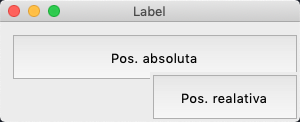
\includegraphics[width=\textwidth]{fig/place1}\\
%\; \\
%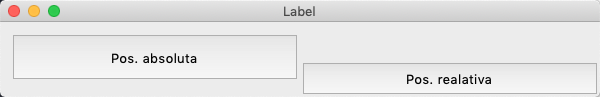
\includegraphics[wideje
%\includegraphics[width=\textwidth]{fig/place3}
%\end{textblock*}
\end{frame}


%%%%%%%%%%%%%%%%%%%%%%%%%%%%%%%%%%%%%
%%%%%%%%%%%%%%%%%%%%%%%%%%%%%%%%%%%%%
\begin{frame}{Ejercicio} 

\begin{ejercicio}{}
?`Qué código se podría escribir para conseguir esta ventana?


\centerline{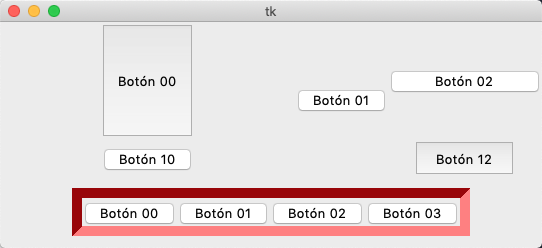
\includegraphics[width=.75\textwidth]{fig/ejercicioGrid}}



\end{ejercicio}

\end{frame}
% . . . . . . . . . . . . . . . . . . . . . . . . . . . . . . . . . . . . . . . . . . . . . . . . . . . . . . 
% . . . . . . . . . . . . . . . . . . . . . . . . . . . . . . . . . . . . . . . . . . . . . . . . . . . . . . 




%%%%%%%%%%%%%%%%%%%%%%%%%%%%%%%%%%%%%
%%%%%%%%%%%%%%%%%%%%%%%%%%%%%%%%%%%%%
\begin{frame}{Ejercicio} 

\begin{ejercicio}{}
Cuál sería la secuencia de instrucciones que permite:

\begin{enumerate}
\item Solicitar el nombre (string) y edad (entero) de $n$-personas.
\item Guardar los nombres y edades en un fichero.
\end{enumerate}

Teniendo en cuenta que:
\begin{enumerate}
\item Será obligatorio introducir un string y un entero por persona usando una ventana modal.
\item Se guardarán los datos usando una ventana de diálogo, obligando a introducir el nombre de dicho fichero.
\end{enumerate}

No es necesario crear clases, solo escribir la secuencia de instrucciones.

\end{ejercicio}

\begin{ejercicio}{}
Construye una calculadora simple: consta de dos entradas donde se introducen dos valores reales y un botón que al ser pulsado lee los valores de ambos campos para volcar el resultado en otro campo (no editable).

Escribe primero la secuencia de instrucciones y posteriormente escribe la versión en la que la calculadora es una clase hija de Tkinter.
\end{ejercicio}

\end{frame}
% . . . . . . . . . . . . . . . . . . . . . . . . . . . . . . . . . . . . . . . . . . . . . . . . . . . . . . 
% . . . . . . . . . . . . . . . . . . . . . . . . . . . . . . . . . . . . . . . . . . . . . . . . . . . . . . 




%%%%%%%%%%%%%%%%%%%%%%%%%%%%%%%%%%%%%
%%%%%%%%%%%%%%%%%%%%%%%%%%%%%%%%%%%%%
\section{Lugares de Interés}


%%%%%%%%%%%%%%%%%%%%%%%%%%%%%%%%%%%%%
%%%%%%%%%%%%%%%%%%%%%%%%%%%%%%%%%%%%%
\begin{frame}{Referencias}
Algunos lugares de referencia \key{para consultar} sobreTkinter: 

\begin{itemize} \footnotesize
\item \url{https://python-course.eu/python_tkinter.php}
\item \url{https://docs.python.org/3.9/library/tkinter.html}
\item \url{https://zetcode.com/tkinter/}
%\item \url{https://guia-tkinter.readthedocs.io/es/develop/}
\item \url{https://python-para-impacientes.blogspot.com/2016/02/variables-de-control-en-tkinter.html}
\item \url{https://tkdocs.com/tutorial/widgets.html}
\item \url{https://docs.hektorprofe.net/python/interfaces-graficas-con-tkinter/}
\item \url{https://youtube.com/playlist?list=PLU8oAlHdN5BlvPxziopYZRd55pdqFwkeS}
\item \url{http://www.java2s.com/Code/Python/GUI-Tk/CatalogGUI-Tk.htm}
\end{itemize}

\end{frame}


\end{document}




%%%%%%%%%%%%%%%%%%%%%%%%%%%%%%%%%%%%%
%%%%%%%%%%%%%%%%%%%%%%%%%%%%%%%%%%%%%
\begin{frame}[fragile]{Widgets Básicos}
\begin{itemize}

\item Label: \pyv{label = tk.Label(parent, text='Full name:')}. 

Se pueden mostrar imágenes:
	
\begin{pyverbatim}
image = PhotoImage(file='myimage.gif')
label['image'] = image
\end{pyverbatim}

\item Buttom \pyv{button = tk.Button(parent, text='Okay', command=submitForm)}

\item Checkbutton: 

destructFlag = StringVar()
cb = tk.Checkbutton(parent, text="Self-destruct on close", 
   variable=destructFlag)
check = tk.Checkbutton(parent, text='Use Metric', 
	    command=metricChanged, variable=measureSystem,
	    onvalue='metric', offvalue='imperial')
   
   
\end{itemize}
\end{frame}



\end{document}




